% !TEX root = ../Диплом.tex

\section{Квадратизация} \label{sec:quadratiaztion}

\begin{definition}
    Процесс преобразования нелинейных систем \ref{eq:ODE-norm-system}, \ref{eq:ADE-system} к квадратичному виду будем называть \textit{квадратизацией}.
\end{definition}

В данном разделе мы будем рассматривать оригинальные алгоритмы квадратизации, применимые только для  полиномиальных систем \cite{Gu-PhD}. Мы уже описали способы получения таких систем из систем \ref{eq:ODE-norm-system}, \ref{eq:ADE-system} в секции \ref{sec:polynomialization}. Так же заметим, что подходы, применяемые для квадратизации систем, весьма похожи на методы полиномиализации.

\subsection{Квадратизация с помощью введения алгебраических уравнений} \label{sec:quad-algebraic}

Данный алгоритм квадратизует систему, добавляя к ней алгебраические уравнения.

\begin{enumerate}
    \item Ввести новую переменную $y_i = m_i(\vec x)$, где $m_i(\vec x) = x_1^{b_1}\cdot \cdots \cdot x_n^{b_n}$ - моном, образованный из переменных системы.
    \item Заменить $m_i(\vec x)$ на $y_i$ в оригинальном уравнении.
    \item Добавить новое уравнение $y_i = m_i(\vec x)$ в систему.
\end{enumerate}

Показанный алгоритм приводит полиномиальные системы вида \eqref{eq:ODE-norm-system}, \eqref{eq:ADE-system} к квадратичным системам вида \eqref{eq:ADE-system}.

\begin{example}
    Квадратизуем систему, полученную в примере раздела \ref{sec:poly-algebraic}:

    $\begin{array}{lcl}
        \dot x = x^3 + y_1 \\
        0 = xy_1 + y_1 - 1
    \end{array}$
    \newline
    
    Теперь проведём квадратизацию:
    
    \begin{enumerate}
    	\item Вводим новую переменную $y_2 =  x^2$
    	\item Делаем замену в первом уравнении $\dot x = xy_2 + y_1$
    	\item Добавляем новое уравнение в систему $y_2 - x^2 = 0$
    \end{enumerate}
    
    Получили квадратичную систему
    
    $\begin{array}{lcl}
        \dot x = xy_2 + y_1 \\
        0 = xy_1 + y_1 - 1 \\
        0 = y_2 - x^2
    \end{array}$
\end{example}


\subsection{Квадратизация с помощью введения дифференциальных уравнений} \label{sec:quad-diff}

Следующий алгоритм проводит квадратизацию, добавляя в систему ОДУ:

\begin{enumerate}
    \item Ввести новую переменную $y_i = m_i(\vec x)$, где $m_i(\vec x) = x_1^{b_1}\cdot \cdots \cdot x_n^{b_n}$ - моном, образованный из переменных системы.
    \item Заменить $m_i(\vec x)$ на $y_i$ в оригинальном уравнении
    \item Добавить новое уравнение $\dot y_i = \dot {m_i}(\vec x) = m'_i(\vec x) \dot{\vec x}$ в систему, где $m'(\vec x) = \frac {dm(\vec x)}{d \vec x}$
\end{enumerate}

Данный алгоритм переводит полиномиальные системы к квадратичному виду, не меняя их структуры: \eqref{eq:ODE-norm-system} $\longrightarrow$ \eqref{eq:ODE-norm-system}, \eqref{eq:ADE-system} $\longrightarrow$ \eqref{eq:ADE-system}.

\begin{example}
    Рассмотрим систему

    $\begin{array}{lcl}
        \dot x = xz^2 + z \\
        \dot z = x \\
    \end{array}$
    \newline
    
    Теперь проведём квадратизацию:
    \begin{enumerate}
        \item Вводим новую переменную $y = z^2$
        \item Делаем замену в первом уравнении $\dot x = xy + z$
        \item Добавляем новое уравнение в систему $\dot y = 2z \dot z = 2xz$
    \end{enumerate}
    
     Получили квадратичную систему
    
    $\begin{array}{lcl}
        \dot x = xy + z \\
        \dot y = 2xz \\
        \dot z = x \\
    \end{array}$
\end{example}

\subsection{Анализ алгоритмов квадратизации} \label{sec:quad-analysis}

В отличии от полиномиализации, число введённых алгоритмами квадратизации \ref{sec:quad-algebraic}, \ref{sec:quad-diff} уравнений уже не является линейным относительно возможных замен переменных. Более того, как мы покажем далее, число возможных замен так же заметно больше. Поэтому нам становится важен вопрос об оптимальной по числу введённых уравнений квадратизации. Для этого нам понадобится использовать более продвинутые методы анализа, нежели чем для полиномиализации.

Так же заметим, что мы пользуемся только мономиальными заменами, что, вообще говоря, не даёт нам возможности получить оптимальную квадратизацию в общем случае, так как она может достигаться полиномиальными заменами.



\pagebreak

\subsection{Генерация замен переменных}

Генерировать возможные мономиальные замены переменных из монома мы будем рекурсивно, постепенно деля изначальный моном, а далее его мономы из его разложений на все их релевантные делители.

\begin{algorithm}[H]
\SetAlgoLined
\SetKwFunction{FGenRepl}{GenerateReplacements}
\SetKwFunction{FGenReplRec}{GenerateReplacementsRecursive}
\SetKwFunction{FUnique}{Уникальные}
\SetKwFunction{FAdd}{Добавить}
\SetKwFunction{FGenDivs}{СгенерироватьДелители}
\SetKwProg{Fn}{Function}{:}{}
\SetKwData{AllDec}{AllDecompositions}
\SetKwData{monomial}{monomial}
\SetKwData{dec}{decomposition}
\SetKwData{div}{делитель}
\SetKwData{divs}{делители}
\KwData{monomial - входной моном, чьи разложения мы хотим получить.}
\KwResult{Все релевантные разложения монома.}

\Fn{\FGenRepl{\monomial}}{
    \tcc{Множество всех разложений monomial}
    \AllDec = \{\quad\}\;
    \FGenReplRec{\monomial, \{\}, \AllDec}\;
    \Return \FUnique{\AllDec}\;
}
\BlankLine
\BlankLine
\Fn{\FGenReplRec{\monomial, \dec, \AllDec}}{
    \If{\dec не пусто}{
        \FAdd{\AllDec, \dec}\;
    }
    
    \tcc{Генерирует все делители монома степенью не менее 2 и не более $M$ - 1, где $M$ - степень \monomial}
    \divs = \FGenDivs{\monomial}\;
    
    \ForEach{\div: \divs}{
        \FGenReplRec{\monomial / \div, \FAdd{\dec, \div}, \AllDec}\;
    }
    
}
\caption{генерация замен переменных}
\label{algo:Replacement-Gen}
\end{algorithm}

Таким образом, повторив эту процедуру для каждого уникального монома в полиномной системе, мы получим все возможные для неё замены переменных. 

\begin{example}
    $x^2y^3 \Longrightarrow (x, xy^3), (xy, xy^2), (x^2 y^3), (y, x^2 y^2)$ \linebreak $(y, x^2, y^2), (x, xy, y^2), (y^2, x^2 y), (y, xy, xy)$
\end{example}

Заметим, что приведённый алгоритм иллюстрирует лишь идеею получения замен и не является оптимальным способом это делать, так как алгоритм генерирует много эквивалентных разложений, представляющие собой одно и то же разложение, записанное в разном порядке.
\begin{example}
    $(x^2, xy, y^2) \sim (x^2, y^2, xy) \sim (xy, y^2, x^2) \sim \cdots$
\end{example}

Число таких перестановок $P_n - n!$, где $n$ - степень монома. Таким образом, сокращение числа перестановок, которые генерируются алгоритмом \ref{algo:Replacement-Gen}, можно считать главной задачей для его оптимизации. Мы предлагаем в качестве отправной точки попробовать создать дерево, основанное на сжатых префиксных и суффиксных деревьях. Так же, важно заметить, что моном фиксированной степени и числа переменных имеет единственный набор уникальных разложений. Поэтому, можно заранее вычислить все разложения для мономов, часто встречающихся на практике, и использовать их, не вычисляя в момент исполнения программы.

\subsection{Граф замен} \label{replacement-graph-section}

Теперь обобщим процесс выбора замен переменных.

\begin{definition}
    \textit{Граф замен} - ациклический ориентированный граф, чьи вершины представляют системы уравнений, эквивалентные заданной системе, а дуги - преобразования, совершаемые с помощью замены переменной. Входной вершиной мы полагаем заданную систему, а выходной - систему, обладающей нужными нам свойствами.
\end{definition}


\begin{wrapfigure}[12]{l}[10pt]{9cm}
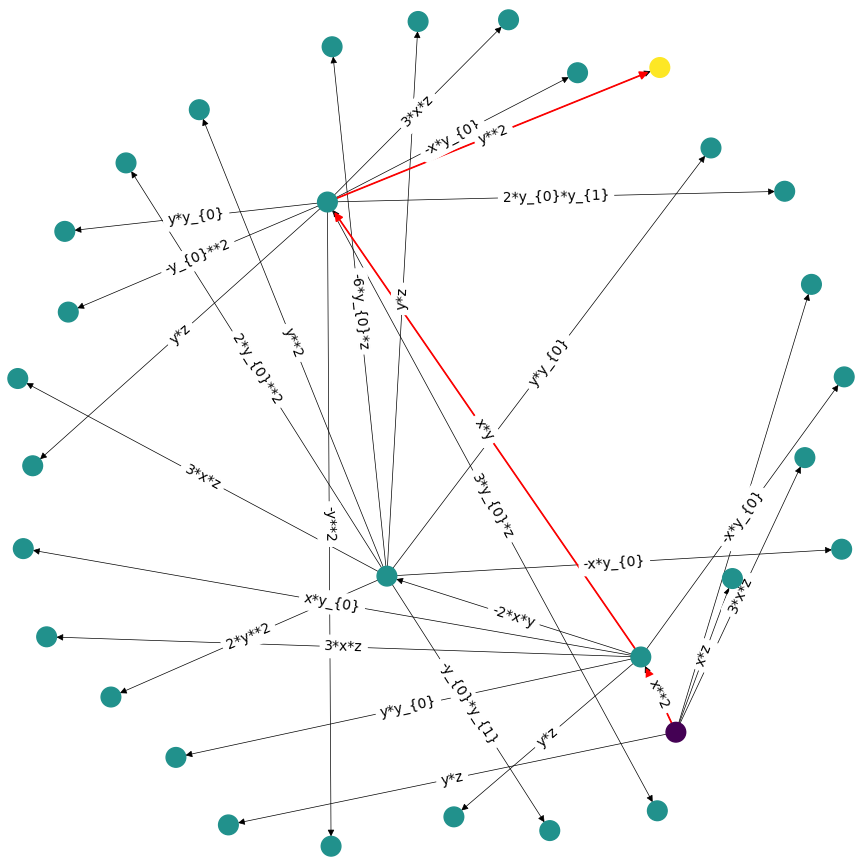
\includegraphics[width=9cm,height=9cm]{chapters/images/replacement_graph.png} 
\caption{Граф замен}
\label{fig:replacement-graph}
\end{wrapfigure}

Таким образом, мы можем трактовать задачу об оптимальной квадратизации как задачу поиска на графе с одним входом и несколькими выходами. Важно заметить, что графы замен, которые нам будут встречаться на практике, часто являются огромными и заранее задан только начальный узел, что делает неприменимыми значительную часть классических алгоритмов поиска.

\subsection{Алгоритмы поиска на графе} \label{search-algo}

В данном разделе мы рассмотрим основные алгоритмы поиска на графе. Подчеркнём, что сам путь нас не интересует, поэтому мы приводим алгоритмы поиска пути на графах, которые, в связи с этим упрощаются.

Пусть $G$ - ориентированный граф, $V$ - множество его рёбер, $E$ - множество его дуг.

\subsubsection{Поиск в глубину (DFS)} \label{DFS-algo}

Поиск в глубину (depth-first search, DFS) заключается в том, что, начиная со стартового узла, исследует его ветви как можно дальше, далее переходя к исследованию других ветвей. Несмотря на то, поиск в глубину применяется в основном при анализе достижимости, он, тем не менее, может находить путь из одной вершины в другую, пусть и не гарантируется то, что найденный путь будет кратчайшим.

\begin{algorithm}[H]
\SetAlgoLined
\SetKwFunction{FDFS}{DFS}
\SetKwProg{Fn}{Function}{:}{}
\KwData{G - входной граф \\
    prop - свойство, которым должна обладать выходная вершина \\
    visited - массив, хранящий для каждой вершины бит, показывающий, посещали ли мы эту вершину}
\KwResult{Вершина, обладающая свойством prop или null, если вершина не найдена}

\Fn{\FDFS{G, v, prop}}{
    visited[v] = true\;
    \If{v обладает свойством prop}{
        \Return v\;
    }
    \ForEach{w: сосед v}{
        \If{visited[w] == false}{
            \Return \FDFS(G, w, prop)\;
        }
    }
    \Return null\;
}
\caption{Поиск в глубину}
\label{algo:DFS}
\end{algorithm}

В худшем случае DFS найдёт искомую вершину последней, поэтому худшая оценка числа операций:
\begin{enumerate}
    \item Чтобы пометить каждую вершину в начале мы посещаем ровно $|V|$ вершин.
    \item В худшем случае мы пройдём по всем дугам графа $|E|$.
\end{enumerate}

Таким образом, число операций в худшем случае можно оценить как $O(|V| + |E|)$

Среднее время работы уже зависит от \textit{prop}.

\subsubsection{Поиск в ширину (BFS)} \label{BFS-algo}

В поиске в ширину (breadth-first search, BFS) граф разбивается на слои: сама входная вершина, вершины на расстоянии 1 от входной вершины, вершины на расстоянии 2 и так далее. Сам поиск исследует слои по возрастанию глубины, пока не найдёт искомую вершину. В отличие от поиска в глубину, BFS всегда отыскивает кратчайший путь до неё.

\begin{algorithm}[H]
\SetAlgoLined
\SetKwFunction{FBFS}{BFS}
\SetKwProg{Fn}{Function}{:}{}
\KwData{G - входной граф \\
    prop - свойство, которым должна обладать выходная вершина \\
    visited - массив, хранящий для каждой вершины бит, показывающий, посещали ли мы эту вершину}
\KwResult{Вершина, обладающая свойством prop или null, если вершина не найдена}

\Fn{\FBFS{G, v_{start}, prop}}{
    \tcc{Очередь из одного элемента}
    Q = \{v_{start}\}\;
    \While{Q не пуста}{
        v = Вытолкнуть(Q)\;
        visited[v] = true\;
        \If{v обладает свойством prop}{
            \Return v\;
        }
        \ForEach{w: сосед v}{
            \If{visited[w] == false}{
                Вставить(Q, w)\;
            }
        }
     }
     \Return null\;
 }
\caption{Поиск в ширину} \label{algo:BFS}
\end{algorithm}

Оценим время работы алгоритма в худшем случае.
\begin{enumerate}
    \item Мы посещаем каждую вершину дважды: в том время, когда мы её помещаем, и при вставке её в очередь: $2|V|$
    \item Каждое ребро в фунции BFS просматривается ровно 1 раз: $|E|$
\end{enumerate}

Таким образом получим оценку $O(|V| + |E|)$, как и у поиска в глубину.

Так же, можно получить альтернативную оценку как числа шагов, так и пространственную сложность в виде $O(b^{d})$, где $b$ - средний коэффициент ветвления графа, $d$- глубина на которой находится выходная вершина. Пусть мы обычно и не знаем $b$ и $d$ точно, но, зная их примерные оценки, мы можем пользоваться данным методом оценки для заранее неисследованных графов.

\subsubsection{Поиск с ограничением глубины (DLS)} \label{DLS-algo}

Поиск с ограничением глубины (depth-limited search, DLS) - вариант поиска в глубину, для которого определяется конечная глубина l на которую он может опуститься. Таким образом, алгоритм всегда работает конечное число шагов, в отличие от DFS, однако ответ не может быть найден, если глубина выходного узла d > l.

\begin{algorithm}[H]
\SetAlgoLined
\SetKwFunction{FDLS}{DLS}
\SetKwProg{Fn}{Function}{:}{}
\KwData{G - входной граф \\
    prop - свойство, которым должна обладать выходная вершина \\
    visited - массив, хранящий для каждой вершины бит, показывающий, посещали ли мы эту вершину \\
    l - предельная глубина}
\KwResult{Вершина, обладающая свойством prop или null, если вершина не найдена}

\Fn{\FDLS{G, v, prop, depth, l}}{
    visited[v] = true\;
    \If{v обладает свойством prop}{
        \Return v\;
    }
    \ForEach{w: сосед v}{
        \If{visited[w] == false \& depth < l}{
            \Return \FDFS(G, w, prop, depth + 1, l)\;
        }
    }
    \Return null\;
}
\caption{Поиск с ограничением глубины} 
\label{algo:DLS}
\end{algorithm}

В худшем случае, число шагов алгоритма оценивается как $O(b^l)$, а пространственная сложность как $O(b \cdot l)$. Таким образом, мы получили лучшие оценки, чем для BFS, при условии, что конечная l выбрана правильно. Гарантировать это поможет следующий алгоритм.

\subsubsection{Поиск в глубину с итеративным углублением (ID-DFS)} \label{ID-DFS-algo}

Поиск в глубину с итеративным углублением (iterative-deepening depth-first search, ID-DFS) запускает DLS на каждой своей итерации и, в случае неудачи, увеличивает конечную глубину l.

\begin{algorithm}[H]
\SetAlgoLined
\SetKwFunction{FIDDFS}{IDDFS}
\SetKwFunction{FDLS}{DLS}
\SetKwProg{Fn}{Function}{:}{}
\SetKwRepeat{Do}{do}{while}
\KwData{G - входной граф \\
prop - свойство, которым должна обладать выходная вершина}
\KwResult{Вершина, обладающая свойством prop или null, если вершина не найдена}

 \Fn{\FIDDFS{G, v_{start}, prop}}{
    l = 1\;
    
    \Do{v == null}{
        v = \FDLS{G, v, prop, 1, l}\;
        l += 1\;
    }
    \Return v\;
 }
\caption{Поиск в глубину с итеративным углублением}
\label{algo:ID-DFS}
\end{algorithm}

Оценкой сложности алгоритма является $O(b^d)$ как у поиска в ширину, а пространственная сложность представляет $O(b \cdot d)$ как у поиска с ограничением глубины, что позволяет ID-DFS использовать преимущества обоих походов.

\subsubsection{Эвристический подход к поиску}

Эвристический поиск, он же информированный поиск представляет собой семейство стратегий поиска,
в котором используются знания о конкретной задаче, зачастую позволяя решать задачу поиска гораздо эффективнее.

Знания о задаче формализуются в качестве эвристических функций.
Эвристические функции сравнивают между собой варианты, из которых алгоритм выбирает следующий шаг.

В случае задач поиска на графе, с помощью эвристических функций мы будем сортировать дуги алгоритмов неинформативного поиска.

Приведём эвристические версии алгоритмов неинформативного поиска
\begin{enumerate}
    \item DFS $\rightarrow$ Поиск по первому наилучшему совпадению (best-first search)
    \item Алгоритм Дейкстры $\rightarrow$ Алгоритм A*
    \item ID-DFS $\rightarrow$ Алгоритм А* с итеративным углублением (Iterative deepening A*, IDA*)
\end{enumerate}


Эвристики, которыми мы будем пользоваться для задачи квадратизации, подробно описаны в секции \ref{heuristics}

\subsection{Алгоритм квадратизации} \label{quad-algo}

\subsubsection{Постановка задачи}

Как мы уже упоминали в разделе \ref{replacement-graph-section}, задача оптимальной квадратизации может быть сформулирована как задача поиска на графе замен. А именно, мы хотим найти квадратичную систему, представляющую собой узел графа замен, так, чтобы найденная квадратичная система находилась на минимальном расстоянии от узла исходной вершины.

Далее рассмотрим известные алгоритмы поиска, приведённые в разделе \ref{search-algo}, в контексте текущей задачи.

\subsubsection{BFS и DFS}

Поиск в глубину и поиск в ширину являются базовыми в задаче поиска, нередко оказываясь достаточно эффективными для многих задач. К сожалению, их в чистом виде достаточно применить для нашей задачи. Действительно, глубина всего графа замен может быть близка к бесконечной при неаккуратном выборе замен, что критично для DFS. В случае BFS нам мешает высокий коэффициент ветвления $b$, который, более того, растёт при для каждого последующего уровня глубины. Таким образом, BFS пригоден для практического использования только в том случае, когда искомая система находится на небольшой глубине. 

\subsubsection{DLS и ID-DLS}

В свете недостатоков BFS и DFS, весьма хорошо смотрится алгоритм поиска с ограничением глубины. Данный алгоритм не уходит дальше заданной глубины, что решает проблему DFS и просматривает узлы на желаемой глубине, а не последовательно идя по слоям, как BFS. Таким образом, при удачно выбранной конечной глубине и хорошем выборе замен на каждом шаге, мы сможем решать задачу за сравнительно небольшое число шагов.

Однако, если мы оценили конечную глубину ниже, чем глубину искомой вершины, то решить задачу мы не сможем. Решает эту проблему алгоритм ID-DFS, который представляет собой DLS, который увеличивает свою конечную глубину в том случае, если искомая вершина не найдена. Недостатком ID-DFS является необходмость исследовать граф заново, если на текущий шаг не нашёл нужную систему. Так же, увеличение глубины всегда происходит только на 1, что не всегда является оптимальной стратегией.

Поэтому мы несколько модифицируем ID-DFS, чтобы устранить данные недостатики. Введём новый алгоритм \textit{Поиск с ограничением глубины с итеративным углублением} (\textit{ID-DLS}), который отличается от ID-DFS в следующем:

\begin{enumerate}
    \item Вместо исследования графа заново после неудачной итерации, ID-DLS сохраняет вершины на текущей конечной глубине вместе с их исходящими заменами. В случае неудачного поиска мы сразу начинаем вычислять неисследованные элементы. Платой за это становится удвоенные затраты на память.
    \item Текущая конечная глубина более гибко изменяется за счёт функции $ОбновитьТекущуюКонечнуюГлубину$. Платой за это становится то, что гарантия оптимальности квадратизации ложится на приведённую функцию. Тем не менее, таким образом мы может искать суб-оптимальные решения с погрешностью, также определяемой функцией $ОбновитьТекущуюКонечнуюГлубину$.
\end{enumerate}

\begin{algorithm}[H]
\SetAlgoLined
\SetKwFunction{FIDDLS}{IDDLS}
\SetKwFunction{FDLS}{DLS}
\SetKwProg{Fn}{Function}{:}{}
\SetKwRepeat{Do}{do}{while}
\KwData{G - входной граф \\
v_{start} - входная вершина \\
prop - свойство, которым должна обладать выходная вершина \\
limit - финальная конечная глубина}
\KwResult{Вершина, обладающая свойством prop или null, если вершина не найдена}

 \Fn{\FIDDLS{G, v_{start}, prop, limit}}{
    currentLimit = 1\;
    
    \tcc{В данную очередь помещаются элементы на текущей конечной глубине вместе с их исходящими заменами. Фактически, мы лениво вычисляем вершины со следующего уровня}
    highDepthQueue = \{\ \}\;
    
    \Do{v == null}{
        \If{currentLimit > limit}{
            \Return null
        }
        v = \FDLS{G, v, prop, 1, currentLimit, highDepthQueue}\;
        currentLimit = ОбновитьТекущуюКонечнуюГлубину(currentLimit)\;
    }
    \Return v\;
 }
\caption{Поиск с ограничением глубины с итеративным углублением}
\label{algo:ID-DLS}
\end{algorithm}



\subsubsection{Выбор эвристик} \label{heuristics}

Точкой ветвления алгоритма квадратизация является шаг, на котором мы выбираем, в какой порядке исследовать возможные замены переменных. Таким образом, определим семейство эвристических функций в задаче квадратизации как 

\begin{equation}
    h:\ \mathbb{M} \longrightarrow \mathbb{R},
\end{equation}
где $\mathbb{M}$ - группа мономов, образованных над переменным $\vec x$ системы \ref{eq:1}. 

\begin{heuristics} \label{FF}
    \textit{Frequent-First}, \textit{FF} - эвристика, выбирающая моном, наиболее часто встречающийся в разложениях. Таким образом, замена переменной затронет наибольшее число мономов в системе.
    
    \begin{example}
        Для разложений $(x^2, xy), (xy, y^2, y^3, xy^2, xy^3), (x^2, y^2, xy)$ мы выберем моном $xy$, так как он встречается в трёх разложениях, а остальные не более чем в двух.
    \end{example}
\end{heuristics}

\begin{heuristics} \label{FVC}
    \textit{Free-Variables-Count}, \textit{FVC} - эвристика, выбирающая моном, образованный из наименьшего числа    переменых. Таким образом, в уравнении $y_i = m'(\vec x) \dot{\vec x}$, соответствующем данной замене, будет минимальное число слагаемых.
    
    \begin{example}
        Из мономов $x^2, xy, xyz$ мы выберем $x^2$, имеющий только одну переменную. Покажем ОДУ, образованные данными заменами:
        \begin{enumerate}
            \item $x^2 \longrightarrow \dot w = 2x \dot x$
            \item $xy \longrightarrow \dot w = \dot x y + x \dot y$
            \item $xyz \longrightarrow \dot w = \dot x yz + x \dot y z + xy \dot x$
        \end{enumerate}
    \end{example}
\end{heuristics}

\begin{heuristics} \label{AED}
    \textit{Auxiliary-Equation-Degree}, \textit{AED} - эвристика, выбирающая моном, порождающий уравнение с наименьшей степенью. 
    
    \begin{example}
        Пусть имеем систему со следующим респределение степеней: $degree(\dot x) = 1,\ degree(\dot y) = 2$. Тогда для замен $x^2, xy, y^2$ получим степени уравнений:
        \begin{enumerate}
            \item $x^2 \longrightarrow \dot w = 2x \dot x \longrightarrow 1 + 1 = 2$
            \item $xy \longrightarrow \dot w = \dot x y + x \dot y \longrightarrow max(1 + 1, 1 + 2) = 3$
            \item $y^2 \longrightarrow \dot w = 2y \dot y \longrightarrow 1 + 2 = 3$
        \end{enumerate}
        Из данных замен выберем $x^2$.
    \end{example}
\end{heuristics}

\begin{heuristics} \label{AEQD}
    \textit{Auxiliary-Equation-Quadratic-Discrepancy}, \textit{AEQD} - эвристика, выбирающая моном, чьё порождённое уравнение наименее отличается от квадратичного. Таким образом, замены, порождающие кважратичные уравнения, имеют самый высокий приоритет. 
    
    \begin{example}
        Пусть имеем замены, порождающие следующие уравнения
        \begin{enumerate}
            \item $m_1 \longrightarrow \dot w = x + y^2 + z^3 \longrightarrow 0 + 0 + 1 = 1$
            \item $m_2 \longrightarrow \dot w = x + y^2 + xy + z^3 \longrightarrow 0 + 0 + 0 + 1 = 1$
            \item $m_3 \longrightarrow \dot w = x + y^2 + z^3 + xyz \longrightarrow 0 + 0 +1 + 1 = 2$
        \end{enumerate}
        Таким образом, $m_1$ и $m_2$ имеют одинаковый приоритет, потому что порождённые ими уравнений имеют минимальную степерь 1.
    \end{example}
\end{heuristics}

\begin{heuristics} \label{AEQD}
    \textit{Summary-Monomial-Degree}, \textit{SMD} - эвристика, представляющая развитие идеи FF. Мы вибираем замену, которая максимально понижает степерь системы.
    
    \begin{example}
        Рассмотрим систему
        
        $\begin{array}{lcl}
             \dot x = xy^2 + y^3 \\
             \dot y = xy + x^2 y + 1
        \end{array}$
        \newline
        
        Понижение степени системы для замены $m$ вычисляетя как $N \cdot (degree(m) - 1)$, где $N$ - число мономов в системе, которые нацело делятся на $m$.
        \begin{enumerate}
            \item $y^2 \longrightarrow 2 \cdot (2 - 1) = 2$
            \item $xy \longrightarrow 3 \cdot (2 - 1) = 3$
            \item $y^3 \longrightarrow 1 \cdot (3 - 1) = 2$
        \end{enumerate}
        Получили, что замена $xy$ максимально сильно снижает степень системы.
    \end{example}
\end{heuristics}

\subsubsection{Правило параллелограмма}

Пусть для начальной полиномиальной системы $S$ имеются две замены $m_1$ и $m_2$.

\begin{wrapfigure}{R}{0.8\textwidth}
\begin{subfigure}{.4\textwidth}
  \centering
  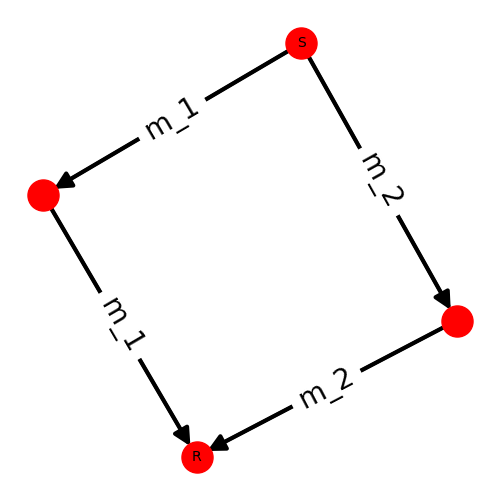
\includegraphics[width=0.8\linewidth]{chapters/images/parallel.png}  
  \caption{Граф замен для $S$}
  \label{fig:parallel-replacement-graph}
\end{subfigure}
\begin{subfigure}{.4\textwidth}
  \centering
  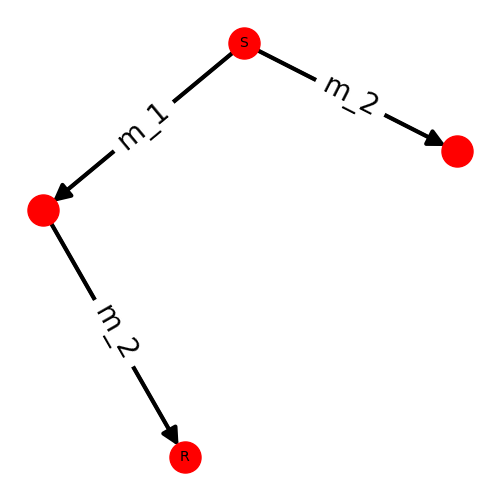
\includegraphics[width=0.8\linewidth]{chapters/images/parallel_red.png}  
  \caption{Упрощённый по правилу параллелограмма граф \ref{fig:parallel-replacement-graph}}
  \label{fig:parallel-replacement-graph-red}
\end{subfigure}
\caption{Правило параллелограмма}
\label{fig:parallel-rule}
\end{wrapfigure}

\begin{proposition}
    Замены $m_1$ и $m_2$ приведут к одной и той же системе $R$ вне зависимости от порядка их проведения. Действительно, ведь в таком случае введённые переменные $y_1$ и $y_2$ получаются перестановкой $[y_1 = y_2,\; y_2 = y_1]$.
\end{proposition}

Таким образом, мы можем убирать часть рёбер из графа во время его исследования. Данная оптимизация становится весьма важна для параллельных версий алгоритма, так как даёт возможность потокам оптимизировать работу друг друга.